\section{Preliminaries}
\label{chp:preliminary}

Throughout the paper, we use the notation $a:A$ to specify a variable of type $A$,  $\mathbf{F}$ to specify a number field, and $\mathbf{F}^{n}$ to specify a multi-dimensional vector with dimension $n$. We denote  by $A \rightarrow B$ the function type from $A$ to $B$ and use $\circ$ for function composition. Moreover, we use $\mathbf{G}[i][j]$ to specify the value of the cell of matrix $\mathbf{G}$ at the $i$-th row and $j$-th column.

\subsection{WASM Run-Time as a State Machine}
\label{chp:exec-trace}
We consider the WASM virtual machine as a gigantic program, with the input as a tuple \initstate, where $\mathbf{I}$ is a WASM executable image that contains a code image $\mathbf{C}$ and an initial memory $\mathbf{H}$, $\mathbf{E}$ is its entry point, and $\mathbf{IO}$ represents the $(\mathbf{stdin}, \mathbf{stdout})$ firmware. In the serverless setup, the WASM run-time starts with an initial state based on the loaded image $\mathbf{I}$, then jumps to the entry point $\mathbf{E}$ and starts executing the bytecode based on the WASM specification. 

Internally the WASM run-time maintains a state $\mathcal{S}$ denoted by a tuple \fullstate \, where $iaddr$ is the current instruction address, $\mathcal{F}$ is the calling frame with a $depth$ field, $\mathcal{M}$ is the memory state, $\mathcal{SP}$ is the stack and $\mathcal{G}$ is the set of global variables. The run-time simulates the semantic of each instruction start at $\mathbf{E}$ until it reaches the exit. The instructions it simulates form an execution trace $\left[t_0, t_1, t_2, t_3, \cdots \right]$ and each transition $t_i$ is a function between states that takes an input $s:\mathcal{S}$ and outputs a new state $s':\mathcal{S}$. For simplicity, we will use the notation of record field to specify a field in state $s:\mathcal{S}$. For example, $s.iaddr$ denotes the current instruction address of state $s$, $s.\mathbf{IO}.\mathbf{stdin}$ denotes the input of state $s$, etc. We also use $op(iaddr)$ to denote the opcode (operation code that specifies the operation to be performed) at address $iaddr$ in the code section $\mathcal{C}$ of image $\mathbf{I}$.

\smallskip Based on the above definition, we define the criteria for a list of state transitions to be valid under \initstate, as follows.

\begin{definition}[Valid Execution Trace]
\label{def:valid-trace}
Given a WASM machine with input \initstate, and $s_0$ is the initial state with $s_0.iaddr = \mathbf{E}$. A valid execution trace is a list of transition functions $t_i$ such that the following holds:
\begin{enumerate}[leftmargin=*]
\item $t_0$ matches the semantic of the instruction $op$ at the entry $iaddr_0 = \mathbf{E}$.
\item For all $k$, $s_k = t_{k-1} \circ \cdots t_1 \circ t_0 (s_0)$, $t_k$ enforces the semantics of $op(s_k.iaddr)$.
\item If $s_{e}$ is the last state, then the depth of the calling frame is zero: $s_e.\mathcal{F}.depth = 0$.
\end{enumerate}
\end{definition}

We take the output of the final state $s_e.\mathbf{IO}.output$ to be the result of the WASM run-time with input \initstate. The $output$ is a valid result if and only if there exists an valid execution sequence $\left[t_0, t_1, \cdots \right]$ such that $s_e$ is the last state of $t_i$ under \initstate.

 
\subsection{Succinct Proof of a Program}

Compared with a standard WASM run-time, \zkwasm\, aims to provide a proof to prove that the output is valid so that it can be used in scenarios which require trustless and privacy computation.  Moreover, the verifying algorithm needs to be simple in the sense of complexity to be useful in practical. Before we dive into how to construct such a proving and verifying scheme for the complex WASM run-time, we go through a few basics about how to construct such a scheme for functions.

Suppose that we have a pure function $f$, a list of parameters $params$ for $f$, an entity $A$ that calculates $r = f(params)$ and an entity $B$ that would like to know $r$ but does not willing to do the exact computation. A scheme that enables $A$ to prove to $B$ about the correctness of $r$ is of great interests in cryptography design if the complexity for $B$ to verify the proof is negligible comparing to the complexity to do the actual calculation. If such a scheme is not interactive and the verifying complexity is negligible comparing to the initial complexity of $f$, then we say it is a SNARK (succinct non-interactive argument of knowledge). If the SNARK proof also leaks no information then it is a ZKSNARK (zero-knowledge succinct non-interactive argument of Knowledge).

\smallskip Topics about constructing \zksnark\, has been well studied in the literature \cite{groth2011efficient, groth2017snarky,groth2016size,groth2017snarky, bootle2016efficient,bunz2018bulletproofs, maller2019sonic, chiesa2020marlin,bunz2020transparent} where functions $f$ are defined by a computational program $\mathbf{P}$.
A common approach for constructing such \zksnark\, is to turn the program $\mathbf{P}:\mathbf{F}^m\rightarrow \mathbf{F}^r$ into a special form of constraint systems $C_i(x) = 0$ (where $C:\mathbf{F}^n \rightarrow \mathbf{F}$), such that for any parameters $param: \mathbf{F}^m$ of $\mathbf{P}$, there exists a unique vector of witness $w:\mathbf{F}^{n-m-r}$ and a unique vector of result $r:\mathbf{F}^r$ that satisfy
\[
C_i(param_0, param_1, \cdots, w_0, w_1, \cdots, r_0, r1, \cdots) = 0.
\]
\noindent We call such constraint system arithmetic circuits (see \ref{chp:arith-circuits} for the precise definition). Once the arithmetic circuits are constructed based on $\mathbf{P}$, the problem of proving $\mathbf{P}(params) = r$ becomes the problems of finding witness vector $w$ and prove that the vector $v = (params;w;r)$ satisfies $C(v) = 0$.
%(see Figure \ref{fig:sum-gates} for an example of constraints on summarize function).
%\begin{figure}[!ht]
%\centerline{
%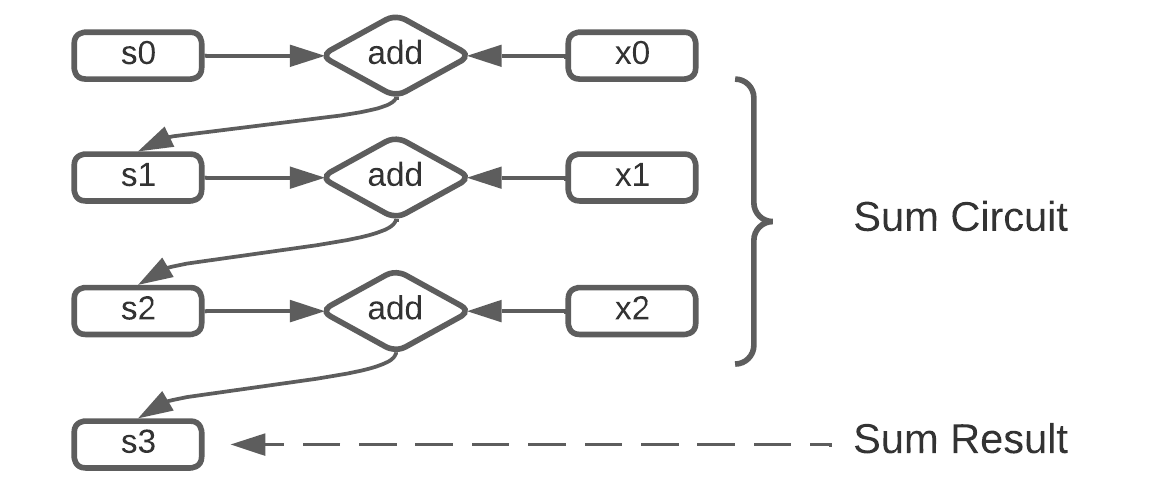
\includegraphics[scale=0.8]{figs/arithment-circuit.png}
%}
%\caption{Arithment Circuit of Sum}\label{fig:sum-gates}
%\end{figure}

Once the problem of constructing \zksnark\, for a program $\mathbf{P}$ is turned into the problem of constructing \zksnark\, for the correspondent constraint system $\mathbf{C}$, various approach can be applied based on the shapes of $\mathbf{C}$. The basic idea to construct \zksnark\, for $\mathbf{C}$ is to turn the proof for the constraint system $\mathbf{C}$ into proofs of polynomial evaluations, that is deriving a list of polynomials $p$ and a list of evaluation pairs $(x_i,v_i)$ such that $\forall i, p_i(x_i) = v_i$ implies $\mathbf{C}$. The technical and implementation details of such transform is not the focus of this paper. We omit the details and give an example to motivate the basic technique behind it.
%which is compressing the list of multi-linear discrete equations in $\mathbf{C}$ into polynomial equations via interpolation.
For example, suppose that a constraint system $\mathbf{C}_i(x) = 0$ can be rewritten into the matrix form $\sum_j c_{ij}x_j = 0$ (linear constraints are used here for simplicity). By Lagrange interpolating on each column vector of $\mathbf{C}$ and vector $x$ we get a list of polynomials $\bar{c}_i(X)$ and $\bar{p}(X)$ such that $\bar{c}_i(j) = c_{ij}$ and $\bar{p}(j) = x_j$. Therefore, $\mathbf{C}_i(x) = 0$ is equivalent to the polynomial equation $\sum \bar{c}_i(X)\bar{p}(X) = 0$ when $X =1,2,3\cdots$. It follows that the proof of $\mathbf{C}$ can be turned into the proof of the polynomial evaluation problem by proving the evaluation of $\sum \bar{c}_i(X)\bar{p}(X) = 0$ at $X=0,1,2\cdots$.

\smallskip A powerful tool for constructing \zksnark\, schemes for the statement of polynomial evaluation is PCS (Polynomial Commitment Schemes \cite{boneh2020halo-pcs,boneh2020efficient-pcs,kate2010polynomial-pcs}). In this paper, without specification, we use KZG (Kate, Zaverucha and Goldberg \cite{kate2010polynomial-pcs}) as our polynomial commitment scheme. Below we will put more efforts on explaining the specific arithmetic circuits we use to describe the semantics of our target program $\mathbf{P}$ which is a WASM virtual machine.

%\subsection{PCS (Polynomial Commitment Schemes)}
%PCS provides a way for the prover and verifier to commit to a polynomial $p$ and then open the commitment at any certain point (prove that the evaluation of $P$ a point $x$ is equal to a claimed value $v$). In this paper, without specification, we use KZG (Kate, Zaverucha and Goldberg) as our polynomial commitment scheme and the commitment formula for a polynomial $p$ is defined by $g^{p(\beta)}$ where $\beta$ is a random value negotiated by prover and verifier at the setup stage and $g$ is a point on a special elliptic curve.

\subsection{Arithmetic Circuits}
\label{chp:arith-circuits}
Arithmetic circuits are a crucial building block in the \zksnark\, of a program. Among various arithmetic circuit systems investigated recently \cite{hoffmann2019efficient-r1cs, gabizon2019plonk, pearson2022plonkup}, we use the Halo2's \cite{halo2book} circuit system for its flexibility in customization and better integration with polynomial lookup which we needed for table lookup and range check.

Based on the arithmetic circuits provided by \zkwasm, the Halo2's zero-knowledge proof system generating execution proofs in a \zksnark\, way. %(\zksnark\, is the abbreviation of Zero-knowledge SNARK which is a scheme that does not only provides a way to generate a succinct proof but also leaks no information). 
The feature of zero-knowledge makes \zkwasm\, extremely useful in scenarios where the prover would like to prove that certain output is calculated from the execution of a particular program image but does not want to leak the data used.

Due to the complicated structure of a full WASM virtual machine, we need to
%Given that the arithmetic circuit is crucial in %building the SNARK of a program and the target program we are trying to tackle is very complicated (a full WASM virtual machine), we need to 
pick a constraint system $\mathbf{C}$ that is rich in expressiveness and fast in proof producing. 

A circuit in Halo2 is defined by a tuple $(\mathbf{G}, \mathbf{C})$ where $\mathbf{G}$ is a $n$ column matrix with rows to be filled later and $\mathbf{C}$ is a set of constraints on a row basis. More precisely, suppose that each cell in $G$ is indexed (relative to a row $l$) as $\mathbf{G}_{l, c, r} = \mathbf{G}[l+r][c]$, then each constraint $\mathbf{C}_i$ in $\mathbf{C}$ is one of the following form 
\begin{equation}
    \mathbf{C}_i(l) = \begin{cases}
        &\mathbf{P} \left(\mathbf{G}_{l, c_0, r_0}, \mathbf{G}_{l, c_1, r_1}, \cdots, \mathbf{G}_{l, c_k, r_k}\right) = 0 \,\,\,\,\,\,\, \textrm{\textbf{or}} \\
        &\left(\mathbf{G}_{l, c_0, r_0}, \mathbf{G}_{l, c_1, r_1}, \cdots, \mathbf{G}_{l, c_k, r_k}\right) \in \mathbf{T}
    \end{cases}
    \label{eq:cs-def}
\end{equation} where $c_k, r_k$ are constants, $\mathbf{P}$ is a fixed multi-linear polynomial and $\mathbf{T}$ is a table. 

\begin{remark}
There are two ways to define constraint in Halo2's constraint system $\mathbf{C}$. One way is using polynomial equations of cells and the other is using polynomial lookup. Polynomial lookup is a special constraint that can enforce that an expression $expr$ of cells belongs to an existing table $\mathbf{T}$. In the rest of the paper, we use the expression $plookup(\mathbf{T}, expr) = 0$ to indicate $expr \in \mathbf{T}$. 
\end{remark}

In the rest of this paper, we use $cur$ as the current row that $\mathbf{C}_i$ is apply on and use the notation $r_i.(cur + r)$ to denote $\mathbf{G}_{cur, i, r}$ to emphasize the column $r_i$. With this notation, we see that the constraint system $\mathbf{C}$ provides a flexible way for us to define constraint of cells of a row and their siblings. For example, given the following summarize function $sum$
\begin{verbatim}
function sum(v) {
    for (suc=0,i=0;i<v.length;i++) {
        suc +=v[i];
    }
    return suc;
}
\end{verbatim}
The circuit for it can be constructed as in Table \ref{tbl:sum-table} and the constraint system enforced on each row is defined in Equation \ref{eq:cs-sum-circuit}.
\begin{table}[!h]
\begin{center}
\caption{Circuit matrix of sum}
\label{tbl:sum-table}
\begin{tabular}{ | c | c | c |}
  \hline
  s & acc & operand \\ 
  \hline
 1 & $sum_0 = 0$ & $v_0$\\
 \hline
 1 & $sum_1 = sum_0 + v_0$ & $v_1$\\
 \hline
 1 & $\cdots$ & $\cdots$\\
 \hline
 0 & $sum_k$ & $nil$\\
 \hline
\end{tabular}
\end{center}
\end{table}

\begin{equation}
 C(cur) = \begin{cases}
     &s.(cur) \times (acc.(cur) + operand.(cur) - acc.(cur+1)) = 0 \\
     &s.(cur) \times (1-s.(cur)) = 0
 \end{cases}
 \label{eq:cs-sum-circuit}
\end{equation}
\begin{remark}
Notice that the first constraint ensures that addition is applied to each row except for the last row, and the second constraint enforces that $s$ is either $1$ or $0$).
\end{remark}

\begin{definition}[Arithmetic Circuit]
The arithmetic circuit is a matrix with $m$ columns equipped with a constraint system $\mathbf{C}$ (as defined in Equation \ref{eq:cs-def}) such that for each row $cur$ in the matrix $\mathbf{C}(cur)$ holds.
\end{definition}


%PCS is polynomialbase, constraint base ---> PCS
\subsection{Connecting ZKWASM Virtual Machine with Arithmetic Circuits}
\label{chp:encode-state-in-circuits}
Now we are ready to make one step further. Instead of constructing a \zksnark\, scheme for simple programs, we would like to construct a \zksnark, for a WASM virtual machine. \zkwasm\,  needs to emulate the execution of $\mathbf{I}$ start with $\mathbf{E}$ under $\mathbf{IO.\mathbf{stdin}}$ to generate $\mathbf{IO.\mathbf{stdout}}$ and provide a \zksnark\, proof which proves that $\mathbf{IO.\mathbf{stdout}}$ is valid. Just like what needs to be done for simple programs to produce a \zksnark, we need to construct a huge arithmetic circuits with carefully designed constraints $\mathbf{C}$ such that the following two are equivalent:
\begin{enumerate}[leftmargin=*]
\item $\mathbf{IO.\mathbf{stdout}}$ is the unique valid output if the execution of $\mathbf{I}$ start with $\mathbf{E}$ under $\mathbf{IO.\mathbf{stdin}}$ satisfies the WASM specification.

\item There exists a list of witness $s_i$ such that $\mathbf{C}(\mathbf{I}, \mathbf{E}, \mathbf{IO}, s_0, s_1,\cdots, s_e) = 0$.
\end{enumerate}

We noticed that a valid execution trace will always produce a valid output respecting the WASM specification. So to construct \zksnark\, for WASM virtual machine, it is sufficient to construct an arithmetic circuit $\mathbf{C}$ of two states before and after an instruction so that the following two are equivalent.
\begin{enumerate}[leftmargin=*]
\item Given $(\mathbf{I}, \mathbf{E}, \mathbf{IO})$ and $s_0$ is the initial state, $\left[t_0, t_1, t_2, \cdots \right]$ is a valid execution trace satisfy Definition \ref{def:valid-trace}.
\item Given an execution trace $\left[t_0, t_1, \cdots \right]$ of $(\mathbf{I}, \mathbf{E}, \mathbf{IO}, s_0)$ and $s_k = t_{k-1} \circ \cdots t_1 \circ t_0 (s_0)$. $\mathbf{C}(\mathbf{I}, \mathbf{E}, \mathbf{IO}, s_k, s_{k+1}) = 0$ implies $t_k$ enforces the semantics of $op(s_k.iaddr)$.
\end{enumerate}

We do not construct such circuit $\mathbf{C}$ from scratch, we construct it from small building blocks in Section \ref{chp:build-blocks} then create the architecture of $\mathbf{C}$ in Section \ref{chp:architecture-circuits} and present all the details in Section \ref{chp:instruction-circuits}.
 
